\msusection{Data Menu}\label{sec:data}
The Data menu in the Program Control window serves two functions: to access images and daily logs.

YCweather is relies on \href{https://one.ubuntu.com/dashboard/}{Ubuntu One} to automatically collect the most recent weather data. For additional details please refer to the YCweather website: \link{aeslaughter.github.com/YCweather}.

\msusubsection{Image Viewer} \label{sec:images}
YCweather contains a basic image viewer for accessing images stored in the YCweather database.  Adding images to the database is explained in Section \ref{sec:add} and the database file structure is explained in Section \ref{sec:advanced}.  To access images, follow these steps:
\begin{enumerate}
	\item Select the station(s) of interest,
	\item Select the start date desired (the end date is not utilized), and
	\item Select Open Images from the Data menu or Toolbar button on the Program Control window.
\end{enumerate}

If images for the selected station(s) exist a window will open displaying the images. One window will appear for each station selected.  Figure \ref{fig:eximage} provides an example of the image window.  In the case where no images exist for selected date, but exist for other dates at this station, an image window will open with the Select Date pop-up menu (see Figure \ref{fig:eximage}) set to the first date available.  

\begin{figure}[ht!]\centering
	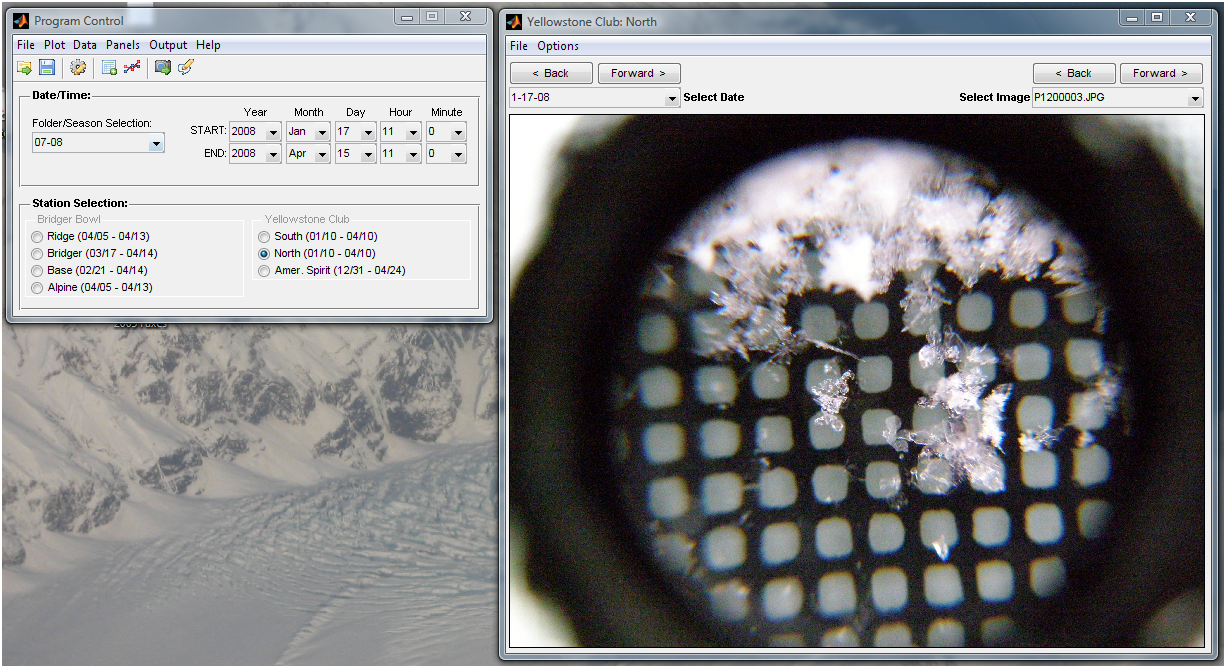
\includegraphics[width=\linewidth]{\YCfiles figures/eximage.png}
	\caption{Example of the image viewer for YCweather.}
	\label{fig:eximage}
\end{figure}

The YCweather image viewer offers the user the following functionality:
\begin{itemize}
     \item Toggles for cycling through images on the current date (right-hand buttons and pop-up menu).
     \item Toggles for changing the date being viewed (left-hand buttons and pop-up menu).
     \item Zooming via the mouse cursor.
     \item The ability to export the figure to another location via the Save image as\ldots ~option in the File menu of the image viewer (this copies the image and does not affect the original).
     \item Capability of renaming an image in the database (Rename in the Options menu).
     \item The ability of using the default Windows-based program for viewing images, which is available as the Open with Windows item in the Options menu. 
\end{itemize}

\msusubsection{Daily Logs} \label{sec:dailylogs}
One of YCweather's main features is the daily logs, which are text notes associated with each station and date.  These logs are stored in the YCweather database (see Section \ref{sec:advanced}) and added via the panel discussed in Section \ref{sec:add}.  Two types of daily logs are available, as shown in Figure \ref{fig:exlog}.  The type of log displayed is controlled in the preferences (Section \ref{sec:pref}).
\begin{enumerate}
	\nitem{Yellowstone Club: } A form specifically designed for usage with a research project at the Yellowstone Club.
	\nitem{General: } A simple form for typing notes.
\end{enumerate}

To open the daily logs: (1) select the station(s) of interest, (2) select the start date desired (the end date is not utilized), and
(3) chose Open Daily Log(s) from the Data menu or Toolbar on the Program Control window.

If daily logs exist then a window, similar to Figure \ref{fig:exlog}, will appear.  The toggles and pop-up menu on the right allow the user to cycle through all the logs for the station.   The daily log may be edited and the changes saved using the Save daily log option in the File menu. Additionally, the log may be opened in a traditional text editor (Open log with Windows in the Open menu); however, this is not recommended for the casual user. Editing the the log in this fashion may render the file unreadable by YCweather.  

It is possible to download images associated with the current station and date of the daily log, this is accessible by selecting Download images from the Open menu.  Finally, the image viewer for the current station may be opened using the daily log window by selecting Open images from the Open menu.

\begin{figure}[ht!]
	\subfloat[Yellowstone Club]{\label{fig:exlogYC}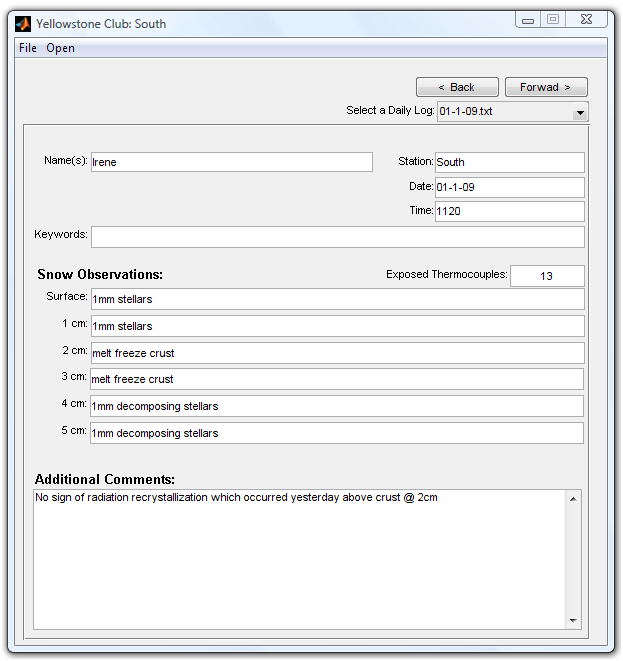
\includegraphics[width=0.49\linewidth]{\YCfiles figures/exlogYC.png}}\quad
	\subfloat[General]{\label{fig:exlogYC}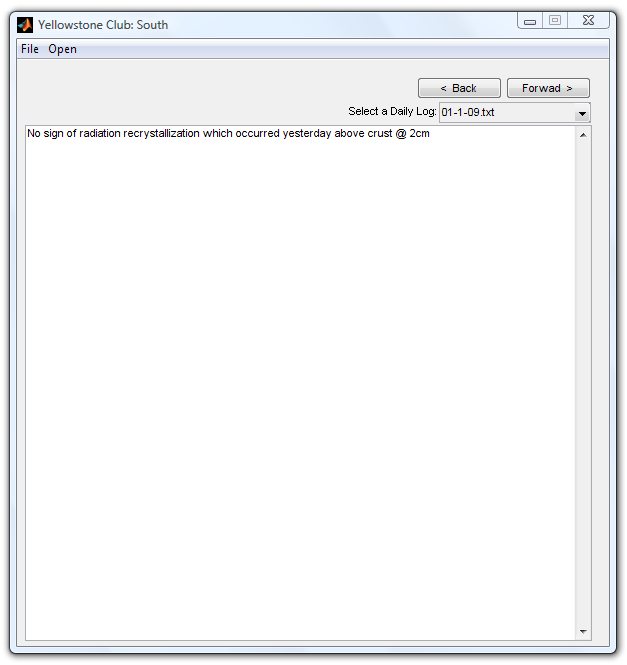
\includegraphics[width=0.49\linewidth]{\YCfiles figures/exlogGN.png}}
	\caption{Examples of the daily log options available in YCweather.}
	\label{fig:exlog}
\end{figure}
